\documentclass{beamer}
%\usepackage{pgfpages}
\setbeameroption{show notes on second screen}

\usepackage{hyperref}
\usepackage{xcolor}
%\usepackage[dvipsnames]{xcolor}
\usepackage{tikz}
\usetheme{Luebeck}
\usecolortheme{magpie}

\definecolor{Turquoise}{rgb}{0.0, 1.0, 0.94}

\beamertemplatenavigationsymbolsempty


\title{Unsupervised Deep Embedding for Clustering Analysis}
\subtitle{Bachelorseminar Data Mining}
\author{Lukas Mahr}
\institute{Ludwig-Maximilians-Universität München}
\date{}


\graphicspath{{images/}}
\setbeamertemplate{headline}{}
\begin{document}

\begin{frame}
\titlepage
\end{frame}


\begin{frame}[plain]{Roadmap}
\tableofcontents[hideallsubsections]
\end{frame}

\section{Clustern von Daten mit hohen Dimensionen}
\begin{frame}[t]{Clustern von Daten mit hohen Dimensionen}\vspace{4pt}
\begin{itemize}
\item Problem
\begin{itemize}
\item Gaussian Mixture Models, KMeans
%\pause
\begin{itemize}
\item Abstandsmetriken sind beschränkt auf den ursprünglichen Datendimensionen
%\pause
\item unwirksam wenn Datendimension hoch sind\cite{steinbach}
%\pause
\end{itemize}
\item Variationen von KMeans für Daten mit hohen Dimensionen
\begin{itemize}
\item limitiert zu linearen Embeddings\cite{ye}
\end{itemize}
%\pause
\item Spectral clustering
\begin{itemize}
\item Quadratische oder Super-quadratische Komplexität
\end{itemize}
\end{itemize}
\item Idee
\begin{itemize}
\item Neuronalesnetzwerk zum reduzieren der Dimensionen
\begin{itemize}
\item nicht lineares mapping
\end{itemize}
\item Clustern der reduzierten Daten
\begin{itemize}
\item einfaches Clustering möglich, da Dimensionen reduziert
\end{itemize}
\item Verbessern des NN und der Cluster durch Backpropagation
\end{itemize}
\end{itemize}

\note{viele Daten Punkte viele Distanzen zu berechnen
schwierig zu visualisieren ohne die Dimensionen zu reduzieren
Komplexität von Kmeans die exponentiell ansteigt}
\end{frame}

\section{Einleitung zu Neuronalen Netzen}
\begin{frame}[t]{Einleitung zu Neuronalen Netzen}\vspace{70pt}
\begin{figure}
\center
\Huge{Neuronale Netze}
\end{figure}
\end{frame}
\subsection{Idee}
\begin{frame}[t]{Einleitung zu Neuronalen Netzen}\vspace{4pt}
\begin{center}
\begin{itemize}
\large\item[] Nicht-lineare statistische Modelle zur Informationsverarbeitung
\large\item[] Informationsverarbeitung umfasst hierbei unter anderem
\begin{itemize}
\item[] Klassifikation
\item[] Prognosenerstellung
\end{itemize}
\large\item[] Units der Neuronalen Netze angelehnt an Neuronen
\begin{itemize}
\item[] Inputs zusammenfassen
\item[] Mit Schwellenwert vergleichen bzw. aktivieren
\end{itemize}
\large\item[] Verbindungen zwischen Units angelehnt an Synapsen
\begin{itemize}
\item[] Gewichtung mit verstärkender oder schwächender Wirkung
\end{itemize}
\end{itemize}
\end{center}
\note{
wofür braucht man neuronale Netze\\
- Klassifizierung von Daten\\
- Prognose eines bestimmten Wertes\\ 
- Neuronen an Neuronen in unserem Gehirn angelehnt\\
- Verbindungen zwischen Künstlichen Neuronen an Synapsen angelehnt\\
- supervised learning = überwachtes lernen\\
-- man besitzt Daten mit Beschriftungen (labels)\\
- unsperviesed learning nicht überwachtes lernen\\
-- unbeschriftete Daten, also es sind keine labels vorhanden\\
}
\end{frame}

    
\subsection{Künstliches Neuron}
\begin{frame}[t]{Einleitung zu Neuronalen Netzen}\vspace{4pt}
Künstlichen Neurons
\begin{figure}
    \centering
        \includegraphics[width=0.8\textwidth]{ArtificialNeuronModel_deutsch_invers.png}
		\tiny\caption{Darstellung eines künstlichen Neurons mit seinen Elementen \tiny\url{https://de.wikipedia.org/wiki/Datei:ArtificialNeuronModel_deutsch.png}}
\end{figure}
\note{
$x_1, ..., x_n$ sind die input variablen, jede der Eingabe variablen besitzt ein
Gewicht, $w_{1j}, ..., w_{nj}$. Diese werden Multipliziert und davon dann die summe berechnet. Hier die Übertragungsfunktion. Dazu wird ein Bias, in dem Fall der Schwellenwert gerechnet. Als letztes gibt es noch die Aktivierungsfunktion die meistens 
einen Wert zwischen 0 und 1 zurückgibt. Das ist dann der input für das nächste Neuron. 
}


\end{frame}

\subsection{Layer/Schicht}
\begin{frame}[t]{Einleitung zu Neuronalen Netzen}\vspace{4pt}
Layer/Schichten
\begin{figure}
    \centering
        \includegraphics[width=0.8\textwidth]{network-layers-invertiert.png}
		\tiny\caption{Deep learning Künstliches neuronales Netz maschinelles lernen Apache MXNet - mehrschichtige PNG \tiny\url{https://de.cleanpng.com/png-x3zkr7/}}
\end{figure}
\note{Layer/Schicht sind mehrere Neuronen die mit allen Neuronen des nächsten Layer/Schicht verbunden sind. Alle Neuronen in einem Layer haben die gleiche Aktivierungsfunktion. Hidden Layer haben meistens die Aktivierungsfunktion rectified linear, da diese recht einfach und schnell zu berchnen ist. Das outputlayer hat meistens eine etwas kompliziertere Funktion wie softmax oder sigmoid. Abhängig von der Aufgabe des Netzwerkes. Letztes Layer hier direkt mit dem Loss}
\end{frame}

\subsection{Aktivierungsfunktion}
\begin{frame}[t]{Einleitung zu Neuronalen Netzen}\vspace{4pt}
Aktivierungsfunktionen
\begin{figure}
    \centering
        \includegraphics[width=0.4\textwidth]{Activation_rectified_linear_invertiert.png}
		\tiny\caption{Rectifier-Aktivierungsfunktion \tiny\url{https://de.wikipedia.org/wiki/Datei:Activation_rectified_linear.svg}}
		\includegraphics[width=0.4\textwidth]{Sigmoid-function_invertiert.png}
		\tiny\caption{Sigmoide Funktion mit Steigungsmaß
		\textcolor{Turquoise}{a}=5 sowie
		\textcolor{yellow}{a} = 10 \tiny\url{https://de.wikipedia.org/wiki/Datei:Sigmoid-function.svg}}
\end{figure}
\note{alles negativ ist wird bei relu zu 0 während bei sigmoid, abhängig von der Steigung Werte zwischen -1 und 1 möglich sind}
\end{frame}


    
\subsection{Loss/Kostenfunktion}
\begin{frame}[t]{Einleitung zu Neuronalen Netzen}\vspace{4pt}
Loss/Kostenfunktion

\begin{figure}

\center

\textbf{Mean Squared Error}\par\medskip
$MSE=\frac{1}{n}\sum^{n}_{i=1}(Y_i - \hat{Y}_i)^2$

\vspace{2em}
\textbf{Mean absolute error}\par\medskip
$MAE=\frac{\sum^{n}_{i=1}|\hat{y_i}- y_i}{n}$

\vspace{2em}
\textbf{Binary Cross-Entropy}\par\medskip
$H(y, \hat{y})=-\frac{1}{n}\sum^{n}_{i=1} y_i\cdot \log({\hat{y_i}}) + (1-y_i)\cdot\log({1-\hat{y_i}}))$
\vspace{1.5em}
\caption{\tiny\url{https://en.wikipedia.org/wiki/Mean_squared_error\#Predictor}
\tiny\url{https://en.wikipedia.org/wiki/Mean_absolute_error}
{\fontsize{5}{6}\selectfont \url{https://towardsdatascience.com/understanding-binary-cross-entropy-log-loss-a-visual-explanation-a3ac6025181a}}
}
\end{figure}
\note{Man berechnet immer den unterschied zwischen den wahren labeln und den predicteden labeln um zu erkenne wie weit diese auseinander liegen. Es wird immer versucht den Loss zu minimieren. Also ein Minimum der Kostenfunktion zu finden.
Die Parameter der Funktion, welche angepasst werden müssen sind alle weights und biases der einzelnen Neuronen und den Layern.}
\end{frame}

\subsection{Backpropagation mit Gradient descent}
\begin{frame}[t]{Einleitung zu Neuronalen Netzen}\vspace{4pt}
Backpropagation mit Gradient descent

\begin{figure}
    \centering
        \includegraphics[width=0.5\textwidth]{1024px-Gradient_descent_invertiert.svg.png}
		\tiny\caption{Illustration of gradient descent on a series of \href{https://en.wikipedia.org/wiki/Level_set}{level sets} \tiny\url{https://en.wikipedia.org/wiki/File:Gradient_descent.svg}}
\end{figure}
\note{Über Backpropagation wird hier mit z.B Gradient Descent die Loass funktion minimiert. Der Gradient der Loss/ Kostenfunktion wird für alle wigths and biases gleichzeitig berechnet. Man kann sich das vorstellen, wie eine Kugel die man einen in einer Hügellandschaft rollen lässt ein kleinen schritten und zwischen den schritten immer nach der Steigung des Abhanges schaut und dabei versucht die Kugel in das tiefste Tal zu bekommen. }
\end{frame}

\section{Autoencoders}
\subsection{Idee}
\begin{frame}[t]{Autoencoders}\vspace{70pt}
\begin{center}
\Huge{Autoencoder}
\end{center}
\note{Ein Autoencoder ist ein feedforward Neural network, was versucht den input zu Kopieren.
Das hört sich im ersten Moment nutzlos an, hat aber doch ein paar Anwendungsmöglichkeiten. Dazu gehört z.B Denosing oder Reduktion des Features Spaces}
\end{frame}

\subsection{Aufbau}
\begin{frame}[t]{Autoencoders}\vspace{4pt}
\begin{figure}
\center
\begin{tikzpicture}
		\node at (0, 0)[](input){Input};
         \node at (2,0) [rectangle,minimum width = 6cm, minimum height = 1cm,rotate=90, draw] (c100) {Encoder};
        \node at (4,0) [rectangle,minimum width = 3cm, minimum height = 1cm,rotate=90, draw] (v100) {Bottleneck};
                 \node at (6,0) [rectangle, minimum width = 6cm, minimum height = 1cm, rotate=90, draw] (v200) {Decoder};
        		\node at (8, 0)[](output){Output};         
        \draw (c100)[-stealth] -- (v100);
        \draw (v100)[-stealth] -- (v200);
        \draw (input)[-stealth] -- (c100);
        \draw (v200)[-stealth] -- (output);
    \end{tikzpicture}
    \caption{Einfaches Autoencoder Model}
\end{figure}
\note{
\begin{itemize}
\item Aufbau, Das Netzwerk besteht im Grunde aus 2 Teilen.
\item Encoder und Decoder
\item Encoder Transformiert die Input Daten in eine kleinere gewünschte Dimension
\item Decoder Transformiert die Daten aus der Kleinen Dimension zurück in die Orginal Dimensionen.
\item Hoffnung das der Encoder die Daten auf die Wichtigsten Features reduziert.
\end{itemize}}
\end{frame}


\begin{frame}[t]{Autoencoders}\vspace{4pt}
\begin{figure}
\center
\includegraphics[scale=0.315]{AutoencoderResult.png}
{\fontsize{5}{6}\selectfont \caption{Orginal und Decoded Bilder}}
\includegraphics[scale=0.315]{DenosingAutoencoderResult.png}
{\fontsize{5}{6}\selectfont \caption{Noisy und Decoded Bilder}}
\end{figure}
\tiny{\url{https://github.com/Plutokekz/dec/blob/main/Autoencoders.ipynb}}
\note{
\begin{itemize}
\item 784 input zu 10 zu 784 (28*28)
\item Bottleneck size = 10 oder feature redutktion auf 10
\item Random noise 
\end{itemize}
}
\end{frame}
\section{Unsupervised Deep Embedding for Clustering Analysis}
\begin{frame}[t]{Unsupervised Deep Embedding for Clustering Analysis}\vspace{45pt}
\begin{figure}
\center
\Huge{DEC}
\\
\vspace{10pt}
\Large{Unsupervised Deep Embedding for Clustering Analysis}

\note{
DEC has two phases: (1) parameter initialization with a deep autoencode\\
parameter optimization (i.e., clustering), where we iterate between computing an auxiliary target distribution and minimizing the Kullback–Leibler (KL) divergence to it.\\
- Besteht aus 2 teilen\\
-- embedding mapping in den kleineren raum Z\\
--- Stacked Autoencoders\\
-- clustering\\
--- Clustern der embddedten Daten 
--- Embeddings verbessern so wie die Cluster anpassen\\}
\end{figure}

\end{frame}
\subsection{Stecked Autoencoders}
\begin{frame}[t]{Stacked Autoencoders}\vspace{4pt}
\begin{figure}
\center
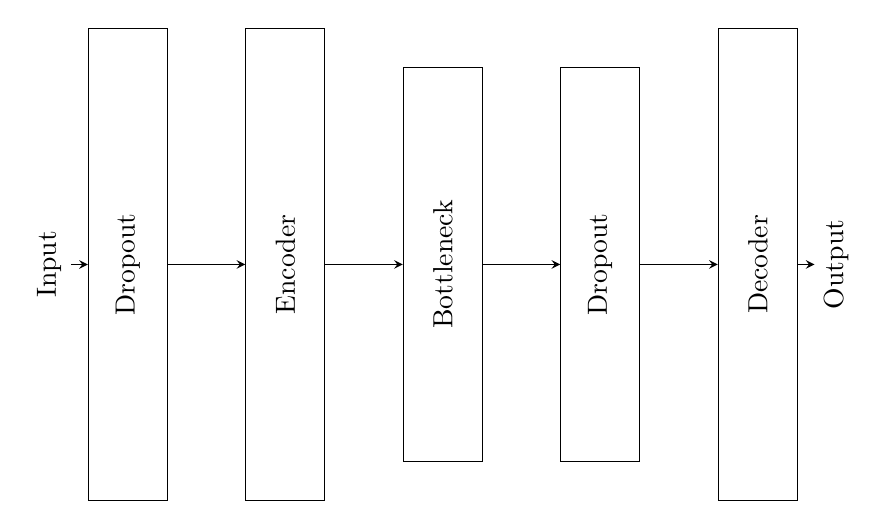
\begin{tikzpicture}
\node at (0, 0)[rotate=90](input){Input};
\node at (1,0) [rectangle,minimum width = 6cm, minimum height = 1cm,rotate=90, draw] (dropout) {Dropout};
\node at (3,0) [rectangle,minimum width = 6cm, minimum height = 1cm,rotate=90, draw] (encoder) {Encoder};
\node at (5,0) [rectangle,minimum width = 5cm, minimum height = 1cm,rotate=90, draw] (bottleneck) {Bottleneck};
\node at (7,0) [rectangle,minimum width = 5cm, minimum height = 1cm,rotate=90, draw] (dropout2) {Dropout};
\node at (9,0) [rectangle, minimum width = 6cm, minimum height = 1cm, rotate=90, draw] (decoder) {Decoder};
\node at (10, 0)[rotate=90](output){Output};         
\draw (input)[-stealth] -- (dropout);
\draw (dropout)[-stealth] -- (encoder);
\draw (encoder)[-stealth] -- (bottleneck);
\draw (bottleneck)[-stealth] -- (dropout2);
\draw (dropout2)[-stealth] -- (decoder);
\draw (decoder)[-stealth] -- (output);
    \end{tikzpicture}
    \caption{Autoencoder mit Dropout}
\end{figure}
\note{
Stacked Autoincoders ist genau das was der name Sagt.\\
mehrere Autoencoder hintereinander.\\
man started mit einem Autoencoder, den man Trainniert.\\
dann entfernt man den decoder Teil\\
und setzt an diese stelle den nächsten Autoencoder, wird wieder trainniert\\
bis die gewünschte anzahl der stacks erreicht ist.\\
Besonderheit man trainiert die folgenden Autoencoder mit dem Output des vorigen encoders.\\
}
\end{frame}

\begin{frame}[t]{Stacked Autoencoders}\vspace{4pt}
\begin{figure}
\center
\begin{tikzpicture}
		\node at (0, 0)[](input){Input};
         \node at (2,0) [rectangle,minimum width = 6cm, minimum height = 1cm,rotate=90, draw] (c100) {Encoder};
        \node at (4,0) [rectangle,minimum width = 5cm, minimum height = 1cm,rotate=90, draw] (v100) {Bottleneck};
       
        \draw (c100)[-stealth] -- (v100);
        \draw (v100)[-stealth] -- (v200);
        \draw (input)[-stealth] -- (c100);
    \end{tikzpicture}
    \caption{Encoder ohne Dropout}
\end{figure}
\note{
Encoder teil ohne noise/dropout und ohne dem decoder\\
}
\end{frame}

\begin{frame}[t]{Stacked Autoencoders}\vspace{35pt}
\begin{figure}
\center
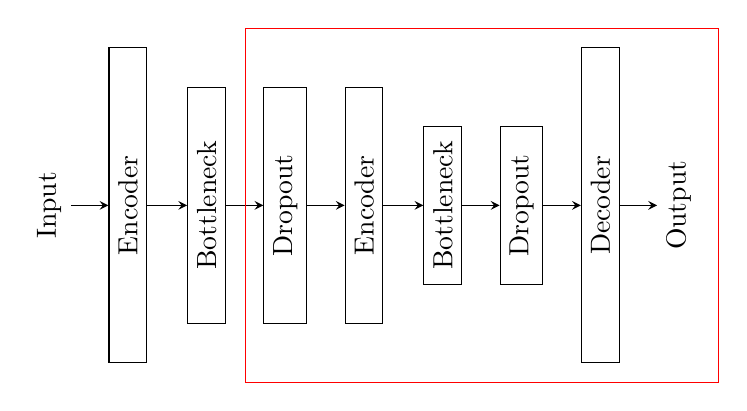
\begin{tikzpicture}
\node at (0.5, 0)[rotate=90](input){Input};
\node at (1.5,0) [rectangle,minimum width = 4cm, minimum height = 0.4cm,rotate=90, draw] (encoder) {Encoder};
\node at (2.5,0) [rectangle,minimum width = 3cm, minimum height = 0.4cm,rotate=90, draw] (bottleneck) {Bottleneck};
\node at (3.5,0) [rectangle,minimum width = 3cm, minimum height = 0.4cm,rotate=90, draw] (dropout0) {Dropout};
\node at (4.5,0) [rectangle,minimum width = 3cm, minimum height = 0.4cm,rotate=90, draw] (encoder2) {Encoder};
\node at (5.5,0) [rectangle,minimum width = 2cm, minimum height = 0.4cm,rotate=90, draw] (dropout) {Bottleneck};
\node at (6.5,0) [rectangle,minimum width = 2cm, minimum height = 0.4cm,rotate=90, draw] (bottlenack2) {Dropout};
\node at (7.5,0) [rectangle, minimum width = 4cm, minimum height = 0.4cm, rotate=90, draw] (decoder) {Decoder};
\node at (8.5, 0)[rotate=90](output){Output};         
\draw (input)[-stealth] -- (encoder);
\draw (encoder)[-stealth] -- (bottleneck);
\draw (bottleneck)[-stealth] -- (dropout0);
\draw (dropout0)[-stealth] -- (encoder2);
\draw (encoder2)[-stealth] -- (dropout);
\draw (dropout)[-stealth] -- (bottlenack2);
\draw (bottlenack2)[-stealth] -- (decoder);
\draw (decoder)[-stealth] -- (output);
\node at (6,0) [rectangle, minimum width = 4.5cm, minimum height = 6cm, rotate=90,color=red, draw] (umrandung) {};
    \end{tikzpicture}
    \caption{Stacked Autoencoder}
\end{figure}
\note{
Aktivierungsfunktion relu außer im letzten Decoder und Encoder Layer sigmoid\\
für die zero-mean imageas\\
Zero-mean images -> durchschnitt pro pixel über alle bilder im Datensatzt\\
das bild wird dann von jedem bild abgezogen und damit liegt der durschnitt bei den Bilder bei null deswegen zero mean images.\\
loss = least-square\\
nach dem Training des Autoencoders wird der Encoder als nicht lineares mapping für die daten genutzt die man Clustern möchte\\
Netzwerk Aufbau input-500-500-2000-10\\
50000 epochs pro layer\\
100000 ganzes Netz ohne dropout epochs fine tuning\\
256 batchsize\\
}
\end{frame}

\section{Deep embedded clustering}
\begin{frame}[t]{Deep embedded clustering}\vspace{70pt}
\begin{figure}
\center
\Huge{Deep embedded clustering}
\end{figure}
\end{frame}

\begin{frame}[t]{Deep embedded clustering}
\begin{figure}
\center
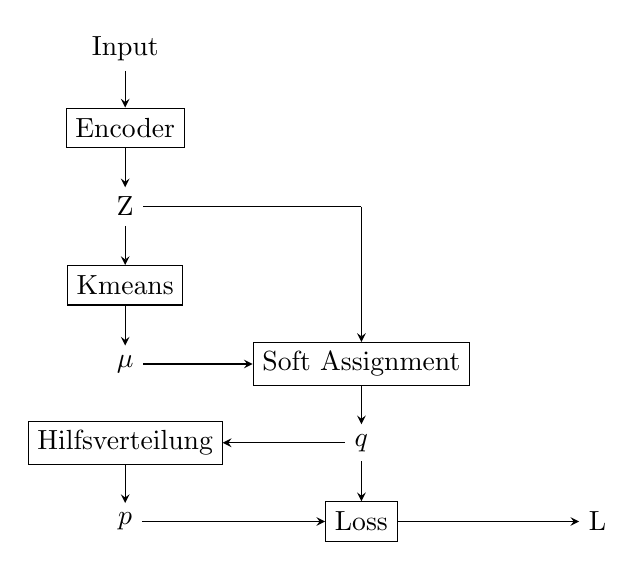
\begin{tikzpicture}
\node [] (input) {Input};
\node [rectangle,minimum width = 0.5cm, minimum height = 0.5cm, draw,below of=input] (encoder) {Encoder};
\node [below of=encoder] (z) {Z};
\node [below of=encoder,xshift=3cm](empty){};
\node [rectangle,minimum width = 0.5cm, minimum height = 0.5cm, draw,below of=z] (kmeans)
{Kmeans};
\node [below of=kmeans] (mu) {$\mu$}; 
\node [rectangle,minimum width = 0.5cm, minimum height = 0.5cm, draw,below of=kmeans,xshift=3cm] (soft)
{Soft Assignment};
\node [below of=soft] (q) {$q$};
\node [rectangle,minimum width = 0.5cm, minimum height = 0.5cm, draw,below of=mu] (aux)
{Hilfsverteilung};
\node [below of=aux] (p) {$p$};
\node [rectangle,minimum width = 0.5cm, minimum height = 0.5cm, draw,below of=q] (loss)
{Loss};
\node [below of=q,xshift=3cm] (l) {L};
\draw (input)[-stealth] -- (encoder);
\draw (encoder)[-stealth] -- (z);
\draw (z)[-stealth] -- (kmeans);
\draw (kmeans)[-stealth] -- (mu);
\draw (mu)[-stealth] -- (soft);
\draw (soft)[-stealth] -- (q);
\draw (q)[-stealth] -- (loss);
\draw (q)[-stealth] -- (aux);
\draw (aux)[-stealth] -- (p);
\draw (p)[-stealth] -- (loss);
\draw (z) -- (empty.center);
\draw (empty.center)[-stealth] -- (soft);
\draw (loss)[-stealth] -- (l);
\end{tikzpicture}
\caption{Abstrakter Aufbau des Clustering Layers}
\end{figure}
\note{
- input daten durch sae werden auf kleinen feature raum Z abgebildet\\
- clustern der Daten Z es entstehen die Cluster Schwerpunkte $\mu$\\
- soft assignments zwischen $\mu$ und z, wird zu q\\
- Hilfsverteilung aus q, wird zu p\\
- Loss zwischen q und p\\
}
\end{frame}

\subsection{KMeans}
\begin{frame}[t]{KMeans}\vspace{20pt}
\Huge\begin{figure}
\center
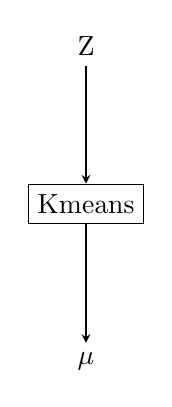
\begin{tikzpicture}
\node at (0,0) (z) {Z};
\node at (0,-2) [rectangle,minimum width = 0.5cm, minimum height = 0.5cm, draw] (kmeans){Kmeans};
\node at (0,-4) (mu) {$\mu$}; 
\draw (z)[-stealth] -- (kmeans);
\draw (kmeans)[-stealth] -- (mu);
\end{tikzpicture}
\end{figure}
\note{
Clustern der Daten aus dem SAE\\
- Cluster Schwerpunkte für Soft Assignment\\
- eigentliche Cluster die man haben will\\ 
}
\end{frame}

\subsection{Soft Assignments}
\begin{frame}[t]{Soft Assignments}\vspace{4pt}
\begin{figure}
\center
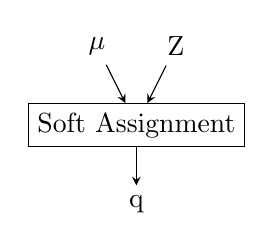
\begin{tikzpicture}
\node at (0,0) (mu) {$\mu$}; 
\node [right of=mu] (z) {Z};
\node [rectangle,minimum width = 0.5cm, minimum height = 0.5cm, draw,below of=mu,xshift=0.5cm] (soft) {Soft Assignment};
\node [below of=soft] (q) {q};
\draw (z)[-stealth] -- (soft);
\draw (mu)[-stealth] -- (soft);
\draw (soft)[-stealth] -- (q);
\end{tikzpicture}
\end{figure}
\begin{figure}
\center
\Huge $q_{ij}=\frac{(1+||z_i-\mu_j||^2/\alpha)^{-\frac{\alpha+1}{2}}}{\sum_{j'}(1+||z_i-\mu_j'||^2/\alpha)^{-\frac{\alpha+1}{2}}}$
\end{figure}
\note{
Student t-Verteilung um die Ähnlichkeit zwischen $z_i$ und $\mu_j$ zu messen\\
Freiheitsgrad ist 1\cite{maaten}\\
$q_{ij}$ ist die Wahrscheinlichkeit die $z_i$  dem Cluster $q_j$ zuzuordnen\\
 
}
\end{frame}

\subsection{Hilfsverteilung}
\begin{frame}[t]{Hilfsverteilung}\vspace{4pt}
\begin{figure}
\center
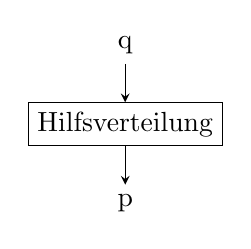
\begin{tikzpicture}
\node at (0,0) (q) {q};
\node [rectangle, draw,below of=q] (aux) {Hilfsverteilung};
\node [below of=aux] (p) {p};
\draw (q)[-stealth] -- (aux);
\draw (aux)[-stealth] -- (p);
\end{tikzpicture}
\end{figure}
\begin{figure}
\center
\Huge $p_{ij}=\frac{q_{ij}^2/f_j}{\sum_{j'}q_{ij'}^2/f_{j'}}$\\
\vspace{10pt}
$f_j=\sum_j q_{ij}$\\
\end{figure}
\note{
Eigenschaften der Hilfsverteilung\\
- Prognosen Verstärken\\
- mehr Gewicht auf genaue Datenpunkte\\
- loss Verteilung von jedem Cluster Schwerpunkt normalisieren um zu verhindern das der versteckte Merkmals Bereich nicht verzehrt wird.\\
--- man will das letzte Encoder Layer schützen. \\
$f_j$ Soft-Cluster-Frequenzen\\
Erklärung wie die Eigenschaft erreicht werden im Fazit.\\ 
}
\end{frame}

\subsection{Loss}
\begin{frame}[t]{Loss}\vspace{4pt}
\begin{figure}
\center
\Large Kullback-Leibler-Divergenz
\end{figure}
\begin{figure}
\center
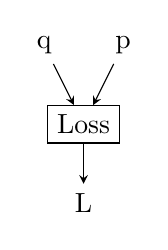
\begin{tikzpicture}
\node at (0,0) (q) {q};
\node [right of=q] (p) {p};
\node [rectangle, draw,below of=q,xshift=0.5cm] (loss) {Loss};
\node [below of=loss] (L) {L};
\draw (q)[-stealth] -- (loss);
\draw (p)[-stealth] -- (loss);
\draw (loss)[-stealth] -- (L);
\end{tikzpicture}
\end{figure}
\begin{figure}
\center
\Huge $L=KL(P||Q)\sum_i\sum_j p_{ij}\log\frac{p_{ij}}{q_{ij}}$\\
\end{figure}
\note{
Kullback-Leibler-Divergenz oder Kullback-Leibler-Abstand\\
- maß für Unterschiedlichkeit zweier Wahrscheinlichkeitsverteilungen\\
- hier als loss funktionen\\
- unterschied zwischen q und p\\
- der unterschied wird versucht zu minimieren.\\
}
\end{frame}

\subsection{Optimierung}
\begin{frame}[t]{Optimierung}\vspace{30pt}
\begin{figure}
\center
\Large Stochastic Gradient Descent
\end{figure}
\vspace{20pt}
\begin{figure}
\Large
\center
$\frac{\partial L}{\partial z_i} = \frac{\alpha+1}{\alpha}\sum_j(1+\frac{||z_i - \mu_j||^2}{\alpha})^{-1}\times (p_{ij}-q_{ij})(z_i-\mu_j)$\\
\vspace{20pt}
$\frac{\partial L}{\partial \mu_j} = -\frac{\alpha+1}{\alpha}\sum_i(1+\frac{||z_i - \mu_j||^2}{\alpha})^{-1}\times (p_{ij}-q_{ij})(z_i-\mu_j)$\\
\end{figure}
\note{
Gradient von L wird berechnet in Abhängigkeit von $q_i$ und $\mu_j$\\
$\frac{\partial L}{\partial z_i}$ wird dann für backpropagation genutzt.\\
wird Optimiert bis eine bestimmter Prozentsatz an Cluster punkten nicht mehr das Cluster wechselt, zwischen zwei fortlaufenden Iterationen.\\
}
\end{frame}

\begin{frame}[t]{Experimente}\vspace{50pt}
\begin{figure}
\center
\Huge
MNIST
\end{figure}
\note{
mnist\\
- 70k Handgeschriebene Zahlen\\
- von 0 - 9\\
- 28*28 pixel\\
}
\end{frame}

\begin{frame}[t]{Experimente}\vspace{50pt}
\begin{figure}
\center
\Huge
STL-10
\end{figure}
\note{STL-10\\
- 10 Klassen\\
- 1300 Bilder pro Klasse\\
zusätzlich:\\
- 100000 Unbeschriftete Bilder\\
- haben beide benutzt\\
- aber gepreprocessed\\
- HOG features mit einem 8*8 filter\\
HOG:\\
- Histogram of Oriented Gradients\\
- Ausrichtung der Kanten und des Gradienten in 8*8 pixel blöcken\\}
\end{frame}

\begin{frame}[t]{Experimente}\vspace{50pt}
\begin{figure}
\center
\Huge
REUTERS
\end{figure}
\note{
Reuters:\\
- 810000 English Nachrichtenberichte\\
- in Kategorie Bäume eingeteilt\\
- 4 Haupt Kategorien (corporate/industrial, government/social, markets, economics)\\
- alle die mehr Haupt Kategorien hatten find raus geflogen\\
- 685071 übrig\\
- tf-idf von den 2000 häufigsten Wort Stämmen\\
- Term Frequency-Inverse Document Frequency\\
- wie wichtig ein Wort in einem Satz von einem Text ist.\\}
\end{frame}

\begin{frame}[t]{Bewertungsmetrik}\vspace{60pt}
\begin{figure}
\center
\Huge
$ACC=\max_m\frac{\sum^n_{i=1} 1\{l_i=m(c_i)\}}{n}$
\note{
- $l_i$ das wahre label\\
- $c_i$ Cluster Zuordnung\\
- $m$ alle one to one Zuordnungen zwischen Clustern und Labels\\
Findet das beste mapping zwischen Cluster und Label
}
\end{figure}
\end{frame}

\begin{frame}[t]{Ergebnisse}\vspace{40pt}
\begin{figure}
\begin{tabular}{l|c|c|c|c}
Methode & MNIST & STL-HOG & REUTERS-10K & REUTERS\\
\hline\hline
k-means & 53.49\% & 28.39\% & 52.42\% & 53.29\%\\
\hline
LDMGI & 84.09\% & 33.08\% & 43.84\% & N/A\\
\hline
SEC & 80.37\% & 30.75\% & 60.08\% & N/A\\
\hline
DEC w/o & 79.82\% & 34.06\% & 70.05\% & 69.62\%\\
\hline
\textbf{DEC} & \textbf{84.30\%} & \textbf{35.90\%} & \textbf{72.17\%} & \textbf{75.63\%}\\
\end{tabular}
\end{figure}
\note{
erklären der anderen Algorithmen und deren Start Bedingungen \\
DEC can process the
entire REUTERS dataset in half an hour with GPU acceler-
ation while the second best algorithms, LDGMI and SEC,
would need months of computation time and terabytes of
memory. We, indeed, could not run these methods on the
full REUTERS dataset and report N/A in Table 2 
}
\end{frame}

\begin{frame}[t]{Clusters}\vspace{20pt}
\begin{columns}
% Column 1
\begin{column}{0.6\textwidth}
    \begin{figure}
    \centering
    \includegraphics[width=0.7\textwidth]{mnist_cluster.png}
    \caption{MNIST}
    \end{figure}
\end{column}
% Column 2    
\begin{column}{0.6\textwidth}
    \begin{figure}
    \centering
    \includegraphics[width=0.7\textwidth]{stl-10_cluster.png}
    \caption{STL-10}
    \end{figure}
\end{column}
\end{columns}
%\caption{Jede Zeile hat die 10 besten Cluster}
\note{
Each row contains the top 10 scoring elements from one cluster.\\
In Fig. 3 we show 10 top scoring images from each clus-
ter in MNIST and STL. Each row corresponds to a cluster
and images are sorted from left to right based on their dis-
tance to the cluster center. We observe that for MNIST,
DEC’s cluster assignment corresponds to natural clusters
very well, with the exception of confusing 4 and 9, while
for STL, DEC is mostly correct with airplanes, trucks and
cars, but spends part of its attention on poses instead of
categories when it comes to animal classes.
}
\end{frame}

\begin{frame}[t]{Autoencoder Features}\vspace{40pt}
\begin{figure}
\center
\begin{tabular}{l|c|c|c|c}
Methode & MNIST & STL-HOG & REUTERS-10K & REUTERS\\
\hline\hline
AE+kmeans & 81.84\% & 33.92\% & 66.59\% & 71.97\%\\
\hline
AE+LDMGI & 83.98\% & 32.04\% & 42.92\% & N/A\\
\hline
AE+SEC & 81.56\% & 32.29\% & 61.86\% & N/A\\
\hline
\textbf{DEC} & \textbf{84.30\%} & \textbf{35.90\%} & \textbf{72.17\%} & \textbf{75.63\%}\\
\end{tabular}
\end{figure}
\end{frame}

\begin{frame}[t]{Gradient Visualisierung}\vspace{4pt}
\begin{figure}
\center
\includegraphics[scale=0.33]{gradient_vs_qij.png}
\caption{Cluster Soft Assignment vs Loss L}
\end{figure}
\note{
Richtigkeit von Hilfsverteilung P und\\
Punkte die nähere am Cluster Mittelpunkt sind haben mehr Einfluss auf den Gradienten.\\}
\end{frame}

\begin{frame}[t]{Cluster Überzeit}\vspace{4pt}
\begin{figure}
\center
\includegraphics[scale=0.35]{ClusterOverTime_tsne_plot.png}
%\caption{•}
\end{figure}
\note{
verbesserung der Cluster über Zeit ??? 

}
\end{frame}

\begin{frame}[t]{Fazit}\vspace{4pt}
?
\end{frame}

\begin{frame}[t]{Von wem ist das Paper}\vspace{30pt}
\begin{figure}
\center
\Large{Junyuan Xie}\\
University of Washington\\
\vspace{8pt}
\Large{Ross Girshick}\\
Facebook AI Research (FAIR)\\
\vspace{8pt}
\Large{Ali Farhadi}\\
University of Washington\\
\end{figure}
\end{frame}


\section{Referenzen}
\begin{frame}[t]{Referenzen}\vspace{4pt}
\begin{thebibliography}{10}
\bibitem{steinbach}
Steinbach, Michael, Ertöz, Levent, and Kumar, Vipin.
The challenges of clustering high dimensional data. In
\textit{New Directions in Statistical Physics,} pp. 273–309. Springer, 2004.

\bibitem{ye}
Ye, Jieping, Zhao, Zheng, and Wu, Mingrui. Discriminative k-means for clustering. In \textit{NIPS}, 2008.

\bibitem{maaten}
van der Maaten, Laurens. Learning a parametric embedding by preserving local structure. In \textit{International Conference on Artificial Intelligence and Statistics}, 2009.
\end{thebibliography}
\end{frame}

\end{document}
